\documentclass[12pt,a4paper]{report}
\usepackage[utf8]{inputenc}
\makeatletter
\usepackage{graphicx}



%Frander Granados Vega
%201117284
%Ingenier\'i­a en Computadores

\pdfinfo{%
  /Title    (Documentaci\'{o}n)
  /Author   (Frander Granados Vega)
}


\begin{document}
\begin{center}
{\LARGE Tecnol\'{o}gico de Costa Rica \\[2 cm]}

{\Large Lenguajes, compiladores e intérpretes \\[3 cm]}

{\Large Ingenier\'{i}a en Computadores \\[3 cm]}

{\Large Primer Proyecto programado \\[3 cm]}

{\large Estudiantes: \\[0.3 cm] }
{\Large Frander Granados 201117284 \\}
{\Large Maikol Barrantes 201230364\\[3 cm]}

{\Large I Semestre, 2015 \\[2 cm] }
\end{center}


\newpage

\begin{flushleft}

1. Manual de usuario: cómo ejecutar el programa, incluir requerimientos de Hardware y Software\\\

El programa fue escrito en scheme utlizando el IDE DrRacket.\\
La función principal es llama "base-datos", para correr el programa basta con correr dicha función de la siguiente manera:\\
(base-datos)\\
Una vez se inicie desplegara un mensaje de bienvenida e información de los comandos a utilizar. En esta sección se explica la forma de uso.\\

La información estará almacenada en “tablas” que son creadas especificando el nombre de la tabla y el nombre de las columnas. El comando ct (crear Tabla) es el primero a explicarse. Crea la tabla estud con los datos carnet, nombre y telefono.\\\

Sintaxis del comando ct:\\
ct estud carnet nombre telefono\\
ct estud2 carnet nombre telefono \\\

La primera columna es el identificador único de la tabla (llave primaria), el cual debe ser diferente para todas las filas que se incluyan en la tabla.\\\

Los datos se incluyen en las tablas por medio del comando ins, insertar, el cual tiene dos formatos. En el primero se indica la tabla en la que se va a 
insertar información, y se incluyen en orden datos para todas y cada una de las columnas de esa tabla Por ejemplo:\\
Sintaxis de ins:\\
ins estud 2012001 julio 5554444\\\

En el segundo formato se indica por medio de una lista el nombre de las columnas que corresponden a los datos incluidos. No es necesario incluir datos para todas las
columnas, pero sí debe haber un dato para el identificador (llave) Por ejemplo:\\
Sintaxis de ins:\\
ins estud (nombre carnet) maria 2010002 \\
ins estud2 (nombre carnet) maria (2012001 True 2012)\\\

La operación sel, seleccionar, localiza en una tabla información que cumpla con la condición especificada. Por ejemplo, la siguiente instrucción.\\
Sintaxis sel:\\
sel matricula (carnet nota) siglaCur ce3104\\\

La operación act, actualizar, permite actualizar valores para una tupla. La operación toma como parámetros el nombre de la tabla, el valor de la 
llave de la tupla que se va a modificar, y una lista de pares nombre-valor con los valores nuevos de las columnas especificadas. Por ejemplo:\\
Sintaxis act:\\
act estud 2012001 nombre julio \\
act estud 2010002 telefono 5557777 nombre marta\\\


\end{flushleft}

\begin{flushleft}

2. Descripción de las estructuras de datos desarrolladas.

\end{flushleft}

\begin{flushleft}
3. Descripción de las principales funciones desarrollados.\\\

Se define un shell llamado consola, (define (consola), esta función tiene un read-line que se guarda en una variable de entrada, dicha variable es analizada
para verificar si es alguno de los comandos definidos.\\
Tiene una condición de parada cuando se escriba "exit".\\
En caso de ingresar un comando valido el programa procede a realizar la operación, verificando primero que la entrada sea string.\\
Este shell le pasa lo captado a una funcion verifica que como dice el nombre nos verifica el comando usado y procede a realizarlo.\\
Para saber que comando se usa "(let ((comando (car(string-split ls))))" con esto se verifica la variable comando que al usar el string-split nos hace la linea
en palabras separadas ejemplo: "hola esto es una prueba"  al aplicarle el string-split $\rightarrow$ "hola" "esto" "es" "una" "prueba" , ya con eso le hacemos car a 
la variable y nos dará el primer elemento, que para el caso de nuestro programa debería ser el comando a usar.\\\

Comando ct:\\
Para este comando se tiene el primer elemento después del comando ct debe ser el nombre de la tabla, para nuestro caso va a ser el nombre del archivo.\\
Se tiene la función y se verifica si va a contener algo o no, en caso de que no vaya a contener nada se crea el archivo vacío, si se van a agregar columnas
se tomas los datos y se pasan a una función auxiliar recursiva, la función escribe en el archivo los datos separados por dos puntos ":", que va a ser nuestro
separador para facilitar las cosas.\\\

Comando isn:\\
Para este comando se debe hacer una validación especial, esto porque el comando puede venir de dos maneras.\\
En la primera se indica la tabla en la que se va a insertar información, y se incluyen en orden datos para todas y cada una de las columnas de esa tabla, como por ejemplo:
"ins estud 2012001 julio 5554444 ", este caso no tiene nada especial.\\
En el segundo formato se indica por medio de una lista el nombre de las columnas que corresponden a los datos incluidos. No es necesario incluir datos para todas las
columnas, pero sí debe haber un dato para la llave como por ejemplo: "ins estud (nombre carnet) maria 2010002 "\\
Para implementar este segundo, se crea una verificación guardando en una variable el tercer elemento\\
(let ((verif(car(cdr(cdr( string-split entrada )))))), el primero corresponde al comando, el segundo a la llave y el tercero puede ser una columna o en este segundo caso es una lista y la sintaxis del comando indica que tiene paréntesis. Tomando esa palabra con el uso de string-ref podemos obtener el elementos que queramos de un string, esta función pasa a char la palabra y nos devuelve el elemento que le indiquemos, ejemplo: la palabra "heisenberg" le aplicamos el string-ref y se obtiene $\#$h $\#$e $\#$i $\#$s $\#$e $\#$n $\#$b $\#$e $\#$r $\#$g, con eso nos daremos cuenta de cual de las dos maneras se esta ingresando. Se verifica en este caso el ejemplo "heisenberg" el primer elemento es la $\#$h para el segundo caso se debería de obtener un paréntesis (. Como restriccion para este comando se debe escribir junto el paréntesis con el dato de la columna ejemplo "ins estud (nombre carnet) maria 2010002" donde el tercer elemento seria (nombre.\\\

Comando act:\\
En este comando se realizan varias cosas, el comando recibe 4 datos, el primero es el archivo o llave, el segundo el ID que se desea actualizar, en caso 
de que el ID no exista se devuelve un mensaje indicando al usuario que no existe el ID.\\
El primer paso es borrar el ID de la tabla para luego agregarlo nuevamente con los datos nuevos.\\\


\end{flushleft}

\begin{flushleft}

4. Problemas conocidos: En está sección se detalla cualquier problema que no se ha podido solucionar en el trabajo.

\end{flushleft}

\begin{flushleft}
5. Actividades realizadas por estudiante: Este es un resumen de las bitácoras de cada estudiante ( estilo timesheet) en términos del tiempo invertido para
una actividad específica que impactó directamente el desarrollo del trabajo, de manera breve (no más de una línea) se describe lo que se realizó, la
cantidad de horas invertidas y la fecha en la que se realizó. Se deben sumar las horas invertidas por cada estudiante, sean conscientes a la hora de
realizar esto el profesor determinará si los reportes están acordes al producto entregado.

Reunión para delegar tareas y procedimiento a seguir con la tarea 25-05-2015 19:00:00 a 20:00:00
Se repasan datos del lenguaje Scheme, se investiga sobre manejo de archivos se inicia 26-05-2015 22:00:00, se finaliza 27-05-2015 00:30:00
Reunion para ver avances 28-05-2015 21:30:00 a 23:00:00
Se realiza shell, un read-line donde acepte los comandos necesarios para el proyecto se inicia 29-05-2015 16:00:00 se finaliza 18:00:00
Se investiga sobre string en scheme en la documentación de DrRacket se inicia 29-05-2015 20:00:00 se finaliza 21:00:00
Se realiza función ct, utilizada para crear tablas se inicia 29-05-2015 22:00:00 se finaliza 30-05-2015 01:00:00 


\end{flushleft}

\begin{flushleft}

6. Corridas de ejemplo: Mostrar los resultados obtenidos al correr la secuencia de comandos que se muestra en la página anterior. En caso de implementación parcial de la tarea mostrar la ejecución de aquellas partes del programa que funcionan.\\

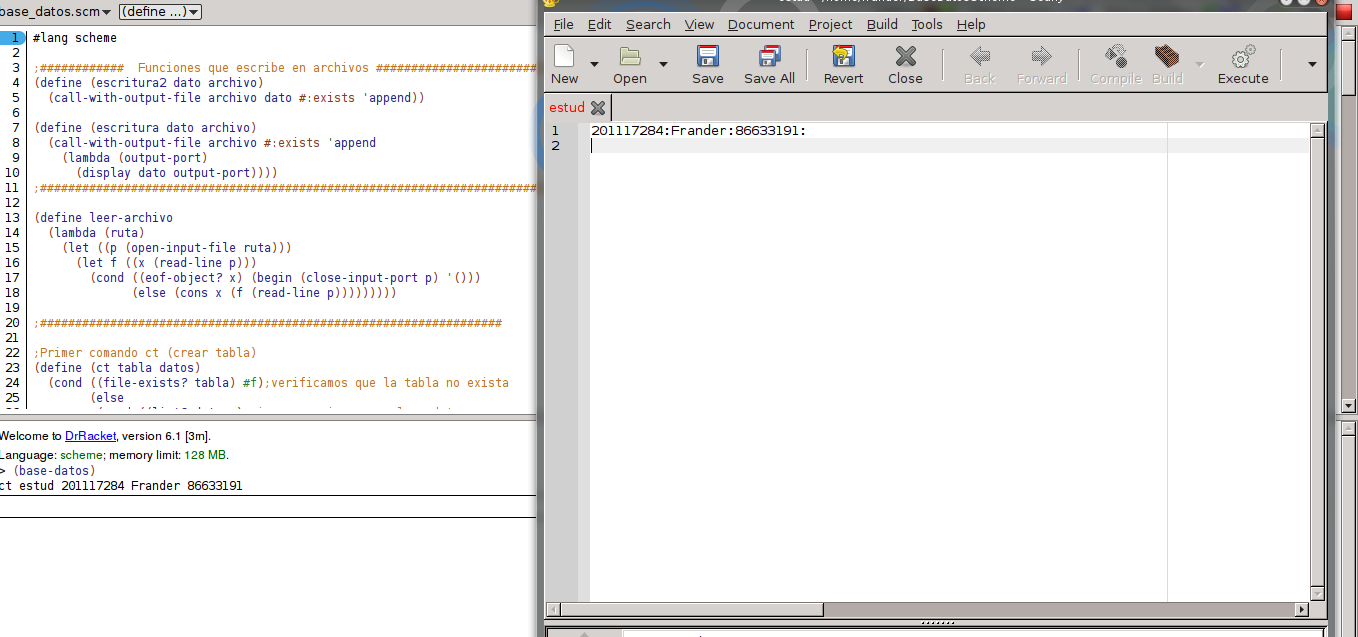
\includegraphics[scale=0.48]{ct1.png} \\\

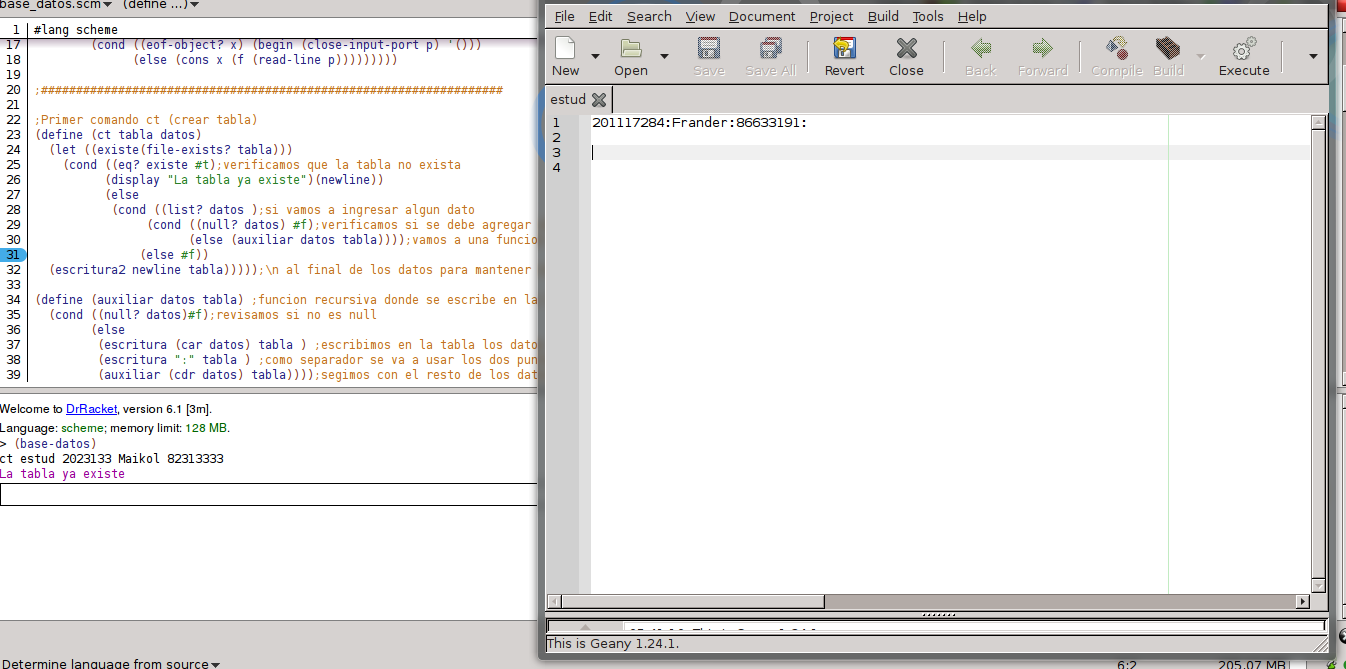
\includegraphics[scale=0.48]{ct2.png} \\\

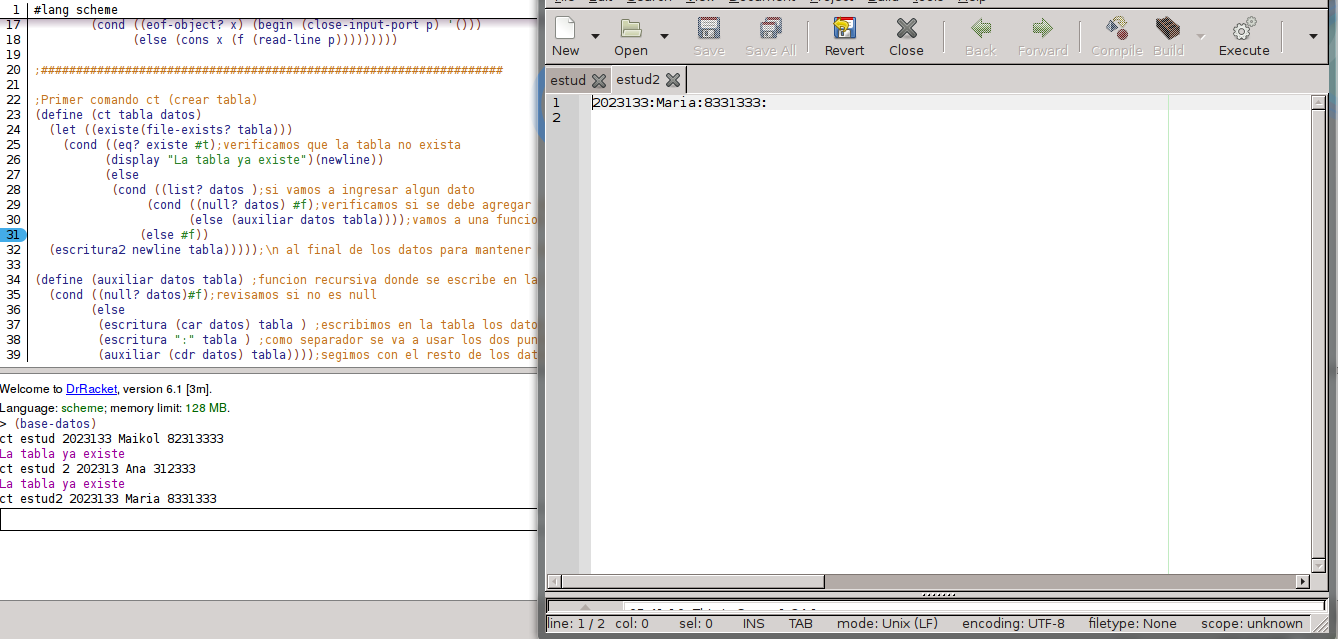
\includegraphics[scale=0.48]{ct3.png} \\\

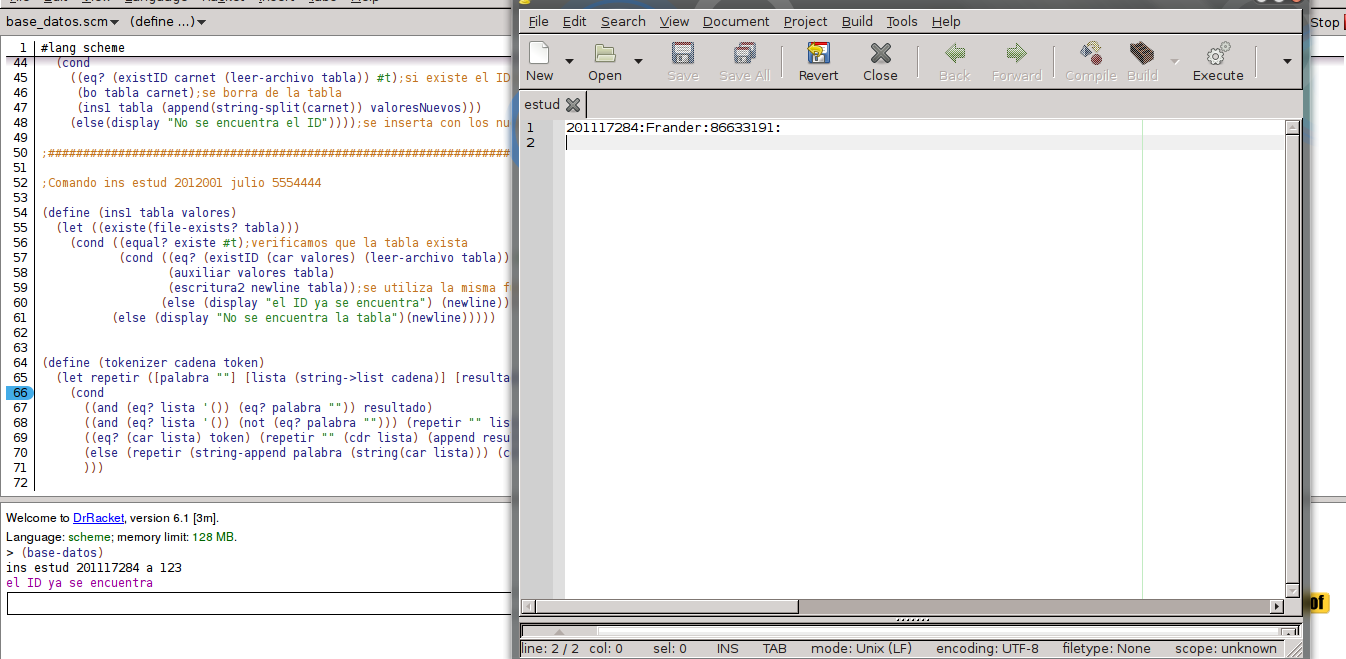
\includegraphics[scale=0.48]{ins1.png} \\\

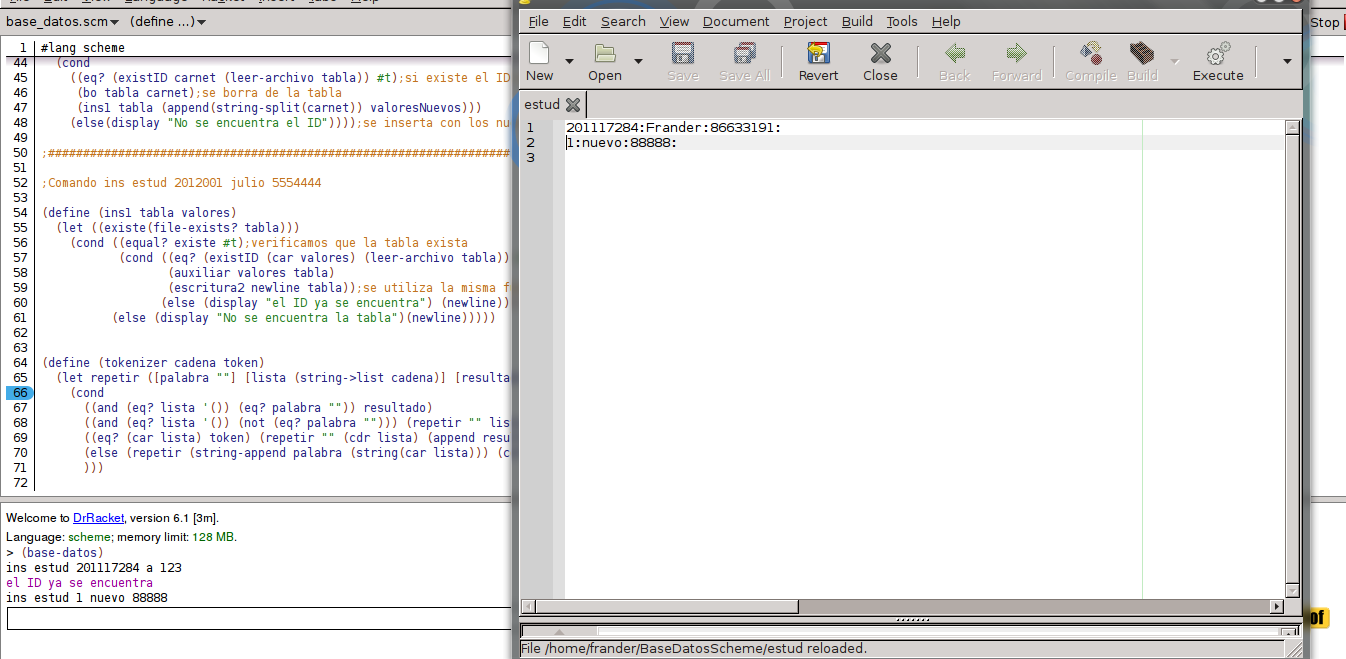
\includegraphics[scale=0.48]{ins2.png} \\\

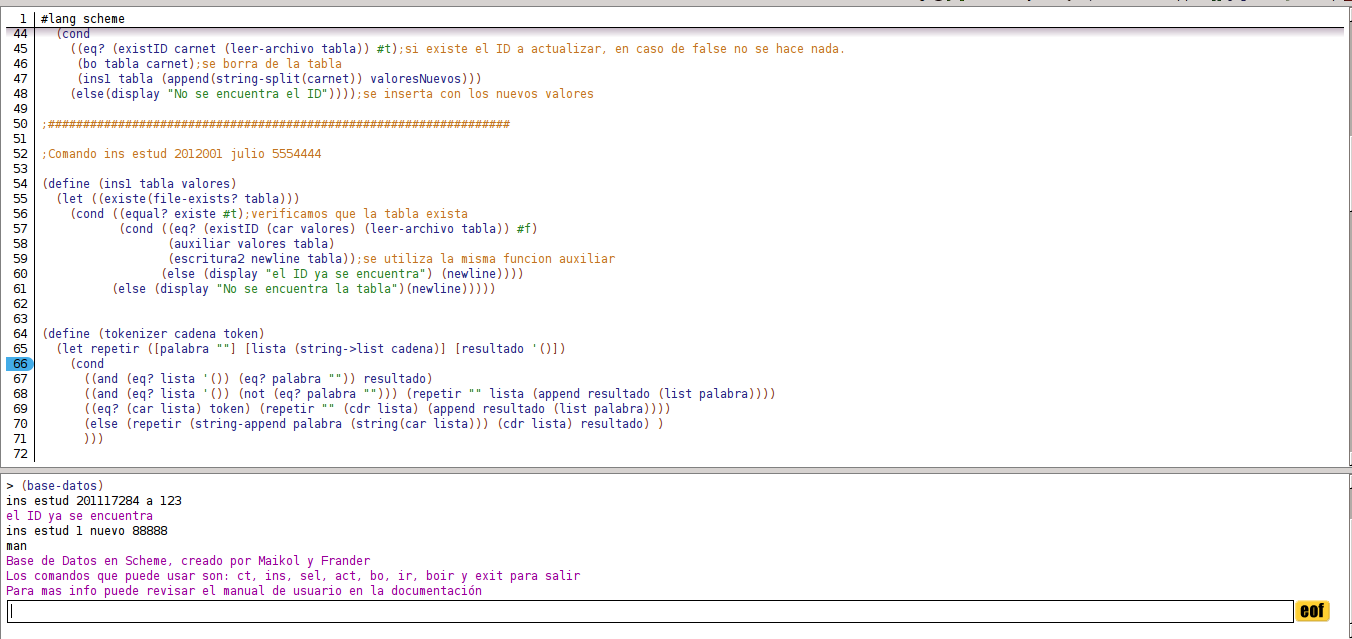
\includegraphics[scale=0.48]{man.png} \\\

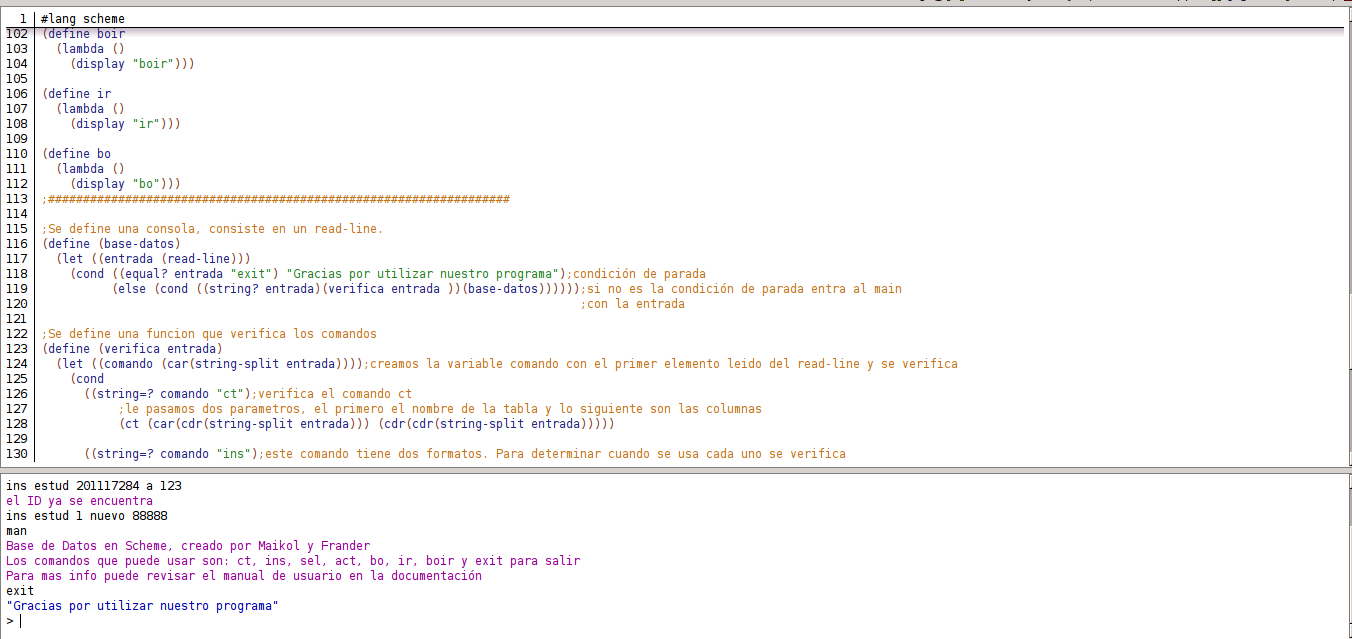
\includegraphics[scale=0.48]{man1.png} \\\

\end{flushleft}

\begin{flushleft}

7. Problemas encontrados: descripción detallada, intentos de solución sin éxito, solución encontradas con su descripción detallada, recomendaciones, conclusiones y bibliografía consultada para este problema específico.

Un problema encontrado fue a la hora de escribir en archivos, el problema es que con la función creada por alguna razón al pasarle un newline 
en lugar de hacer el "$\backslash$n" escribia el proceso newline, ejemplo "\(<\)$\#$procedure:newline\(>\)"\\
Para poder hacer el "enter" al final de cada linea se crea otra función para hacerlo.\\
 


\end{flushleft}

\begin{flushleft}

8. Conclusiones y Recomendaciones del proyecto.

\end{flushleft}

\begin{flushleft}

9. Bibliografía consultada en todo el proyecto




Documentación Racket

Benson, B. (s. f.). 4.3 Strings Recuperado de http://docs.racket-lang.org/reference/strings.html

Benson, B. (s. f.). 4.5 Characters Recuperado de http://docs.racket-lang.org/reference/characters.html$\#$\%$28def.$\_$\%28$\%28quote.$\_$~23$\sim$25kernel$\%$29.$\_$char
$\sim3$f$\%$29$\%$29

Getting a line of user input in Scheme? - Stack Overflow (2010, 04 de Julio). Recuperado de https://stackoverflow.com/questions/3173327/getting-a-line-of-user-input-in-scheme


demas (2011, 07 de Octubre). Scheme - String split function - Stack Overflow Recuperado el 30 de Mayo del 2015, de https://stackoverflow.com/questions/7691769/string-split-function


artofproblemsolving (s. f.). LaTeX:Symbols Recuperado de http://www.artofproblemsolving.com/wiki/index.php/LaTeX%3ASymbols








\end{flushleft}


\end{document}